\documentclass{scrartcl}
\usepackage[utf8]{inputenc}
\usepackage{graphicx}
\usepackage{adjustbox}
\usepackage{amsmath}
\usepackage{float}
\usepackage{siunitx}
\sisetup{
  per-mode=symbol,
  separate-uncertainty
}
\usepackage{hyperref}
\hypersetup{
    colorlinks=true,
    linkcolor=blue,
    filecolor=magenta,      
    urlcolor=cyan,
    pdfpagemode=FullScreen,
    }
\usepackage{authblk}

\usepackage{minted}

\title{CGL-sheet07}

\author[1]{Robin Kühnberger}
\author[2]{Felix Naraschewski}

\affil[1]{University Stuttgart}
\affil[2]{University Stuttgart}

\date{\today}

\begin{document}
\maketitle
\tableofcontents

\section{Numpy-arrays}

\inputminted[breaklines]{python3}{numpy-arrays.py}


\section{Plotten einer gedämpften harmonischen Schwingung mit matplotlib und argparse}

\inputminted[breaklines]{python3}{damped_oscillation.py}

\begin{figure}[H]
	\centering
	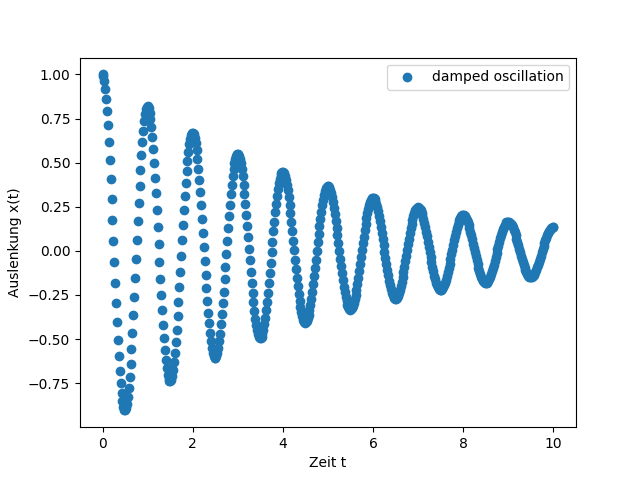
\includegraphics[width=1\textwidth]{damped_oscillation.png}
	\caption{Scatter Plot}
	\label{img:01}
\end{figure}



\section{Array-Slicing}

\inputminted[breaklines]{python3}{array-slicing.py}


%\section*{Quellen}
%\bibliographystyle{plain}
%\bibliography{bibliography}

\listoffigures
%\listoftables

\end{document}